% !TeX spellcheck = ru_RU
% !TEX root = vkr.tex

\section{Экспериментальное исследование}

\subsection{Методология и условия эксперимента}

Экспериментальное исследование проводилось на трёх аппаратных платформах с использованием двух библиотек линейной алгебры: MyGEMM и CLBlast.

\subsubsection{Аппаратные платформы}

\begin{itemize}
    \item \textbf{Banana Pi BPI-F3}: Процессор SpacemiT K1 (8 ядер RISC-V @ 2.0 ГГц), графический процессор IMG BXE-2-32, 16 ГБ LPDDR4-2666;
    \item \textbf{StarFive VisionFive 2}: Процессор JH7110 (4 ядра RISC-V @ 1.5 ГГц), графический процессор IMG BXE-4-32 MC1, 8 ГБ LPDDR4-2800;
    \item \textbf{Intel Core i9-12900H}: Процессор Intel Core i9-12900H (14 ядер @ до 5.0 ГГц), графический процессор Intel Iris Xe Graphics (96 EU), 24 ГБ DDR5-4800.
\end{itemize}

\subsubsection{Программное обеспечение и инструменты}

Для автоматизации тестирования использовался форк репозитория matrix-benchmark~\cite{matrix_benchmark_repo}, включающий:
\begin{itemize}
    \item \texttt{benchmark.sh} -- основной скрипт запуска тестов
    \item \texttt{conf.sh} -- конфигурационный файл с параметрами тестирования
\end{itemize}

Тестирование CLBlast проводилось в двух конфигурациях:
\begin{enumerate}
    \item \textbf{Стандартная сборка} -- библиотека, собранная из исходных кодов с параметрами по умолчанию
    \item \textbf{Тюнингованная версия} -- библиотека, оптимизированная для каждой платформы встроенным тюнером
\end{enumerate}

\subsubsection{Параметры тестирования}

Для обеспечения статистической значимости результатов для каждой конфигурации параметров и каждого ядра выполнялось по 100 прогонов операции умножения матриц для библиотеки MyGEMM и по 10 прогонов для библиотеки CLBlast. Измерялось только время выполнения OpenCL ядра, без учёта времени на подготовку данных.

Основные тестовые данные:
\begin{itemize}
    \item Квадратные матрицы размером $1024 \times 1024$ элементов типа \texttt{float} (сравнительный анализ)
    \item Диапазон размеров матриц от $512 \times 512$ до $7680 \times 7680$ (масштабируемость CLBlast)
\end{itemize}

Для обеспечения стабильности измерений на RISC-V платформах использовалось пассивное охлаждение, частоты процессоров работали в штатном режиме.

\subsection{Тестирование библиотеки MyGEMM}

\subsubsection{Конфигурации параметров}

Тестировались 11 ядер библиотеки MyGEMM с различными наборами параметров конфигурации, адаптированными под ограничения RISC-V платформ:

\begin{itemize}
    \item \textbf{Ядра 1--3}: Параметр TS (Tile Size) со значениями \{8, 16\} (TS=32 вызывал ошибку ``Invalid work group size'')
    \item \textbf{Ядра 4--10}: Комбинации параметров TSM и TSN из множества \{32, 64, 128\} с соответствующими значениями WPTM и WPTN (9 уникальных конфигураций для каждого ядра)
    \item \textbf{Ядро 11}: Фиксированная конфигурация параметров, определённая реализацией clBLAS
\end{itemize}

Все конфигурации были подобраны с учётом ограничения максимального размера рабочей группы в 32 потока на RISC-V платформах.

\subsubsection{Результаты тестирования MyGEMM}

Результаты экспериментов с библиотекой MyGEMM представлены на рисунках~\ref{fig:perf_bananapi}--\ref{fig:perf_intelxe} для каждой из тестируемых платформ.

\begin{figure}[H]
\centering
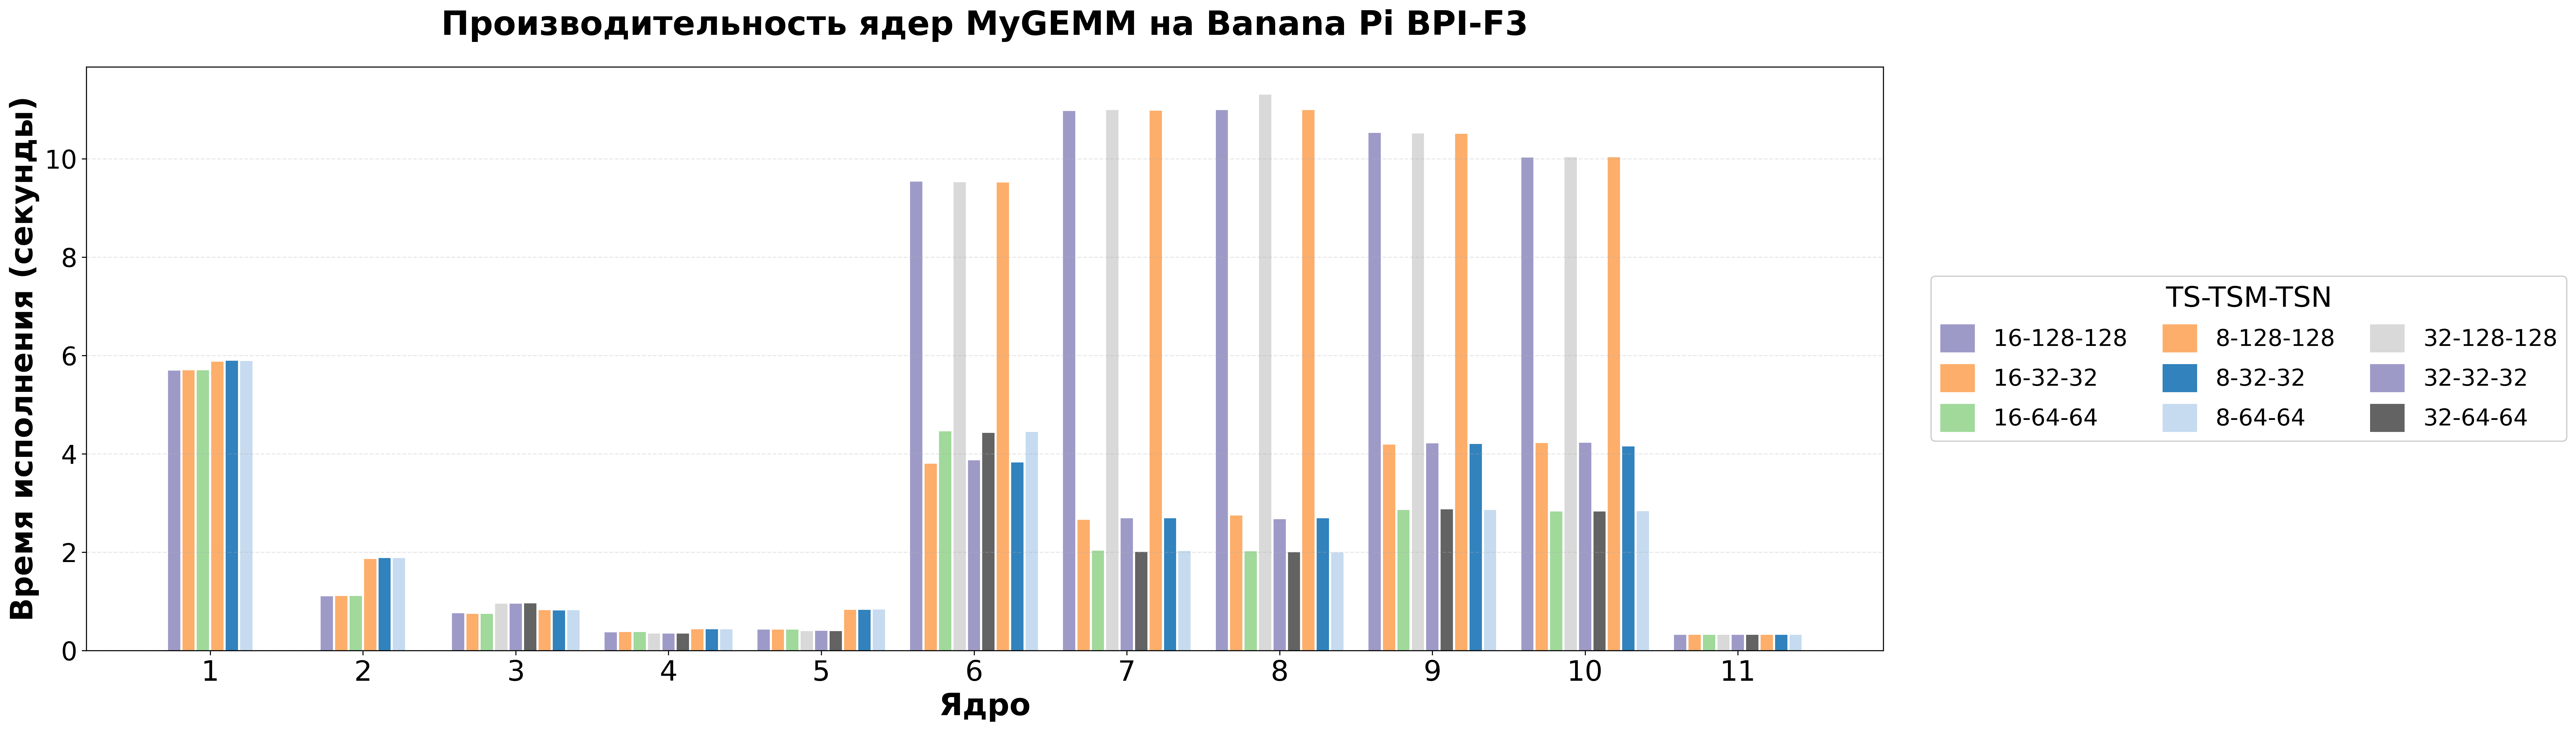
\includegraphics[width=1\textwidth]{figures/banana_pi.png}
\caption{Производительность ядер MyGEMM на платформе Banana Pi BPI-F3}
\label{fig:perf_bananapi}
\end{figure}

\begin{figure}[H]
\centering
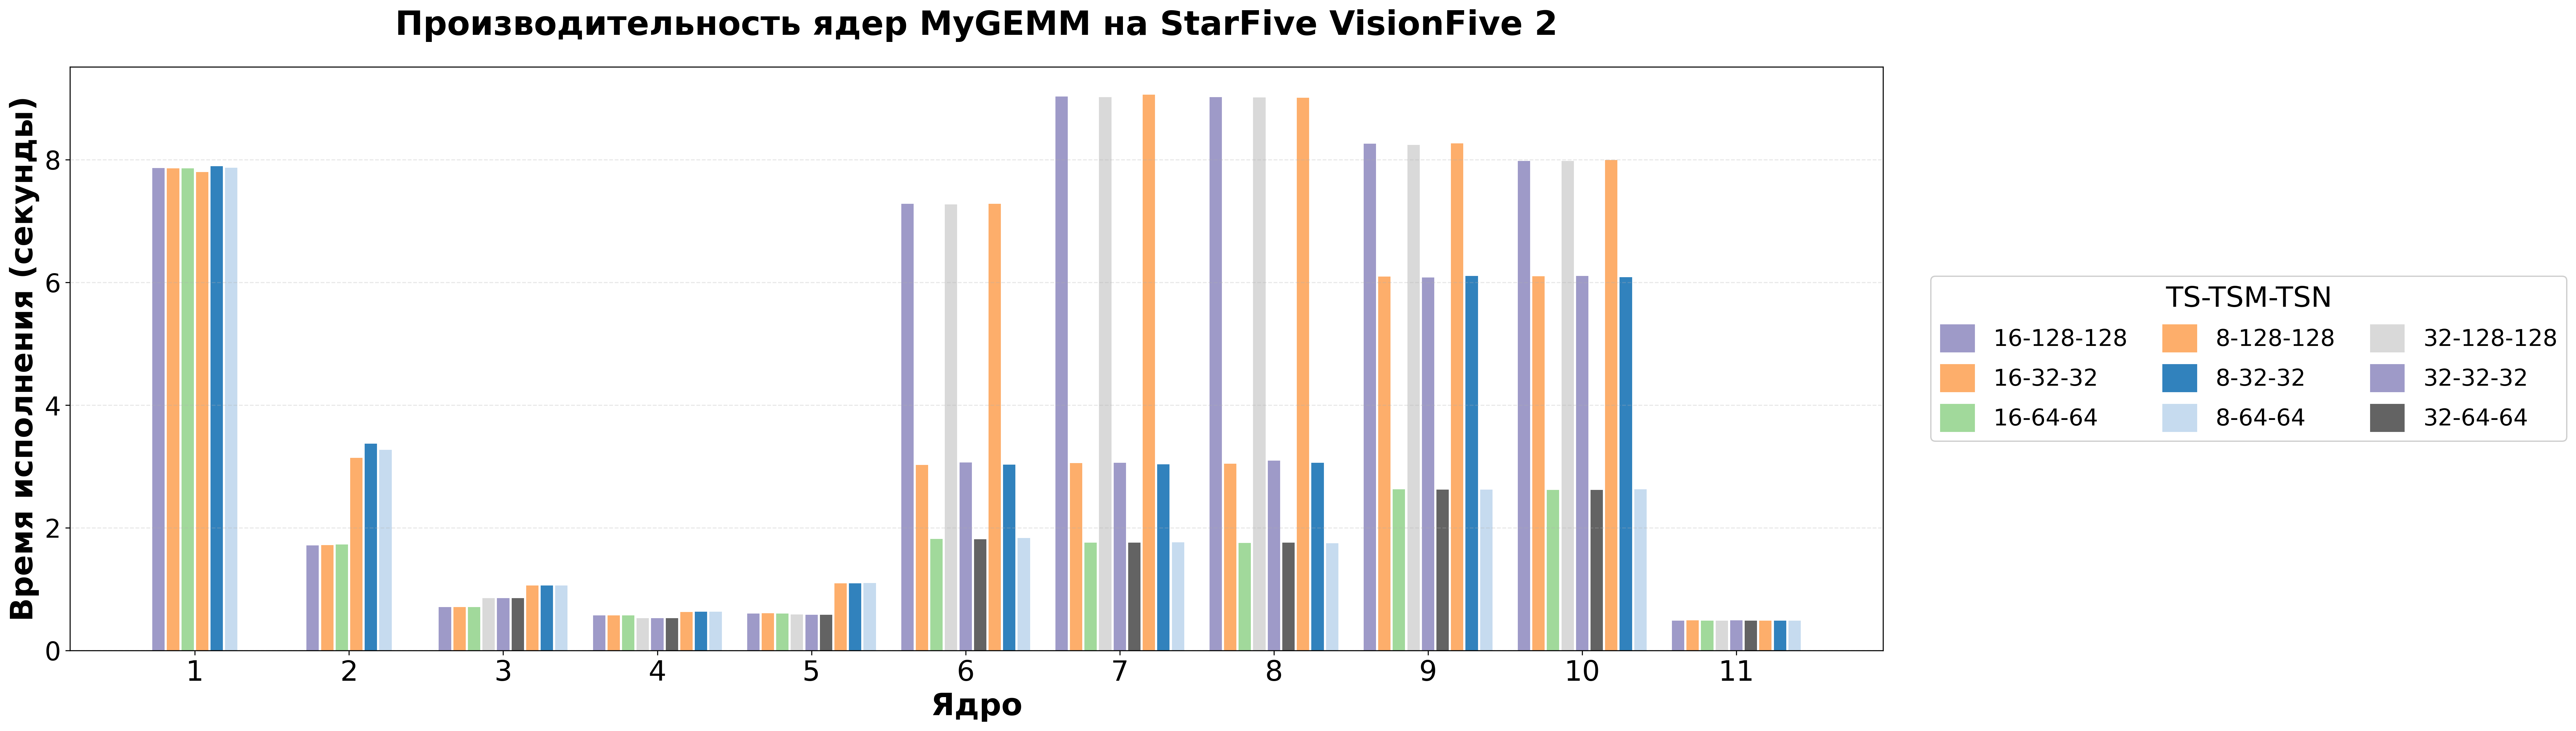
\includegraphics[width=1\textwidth]{figures/starfive.png}
\caption{Производительность ядер MyGEMM на платформе StarFive VisionFive 2}
\label{fig:perf_starfive}
\end{figure}

\begin{figure}[H]
\centering
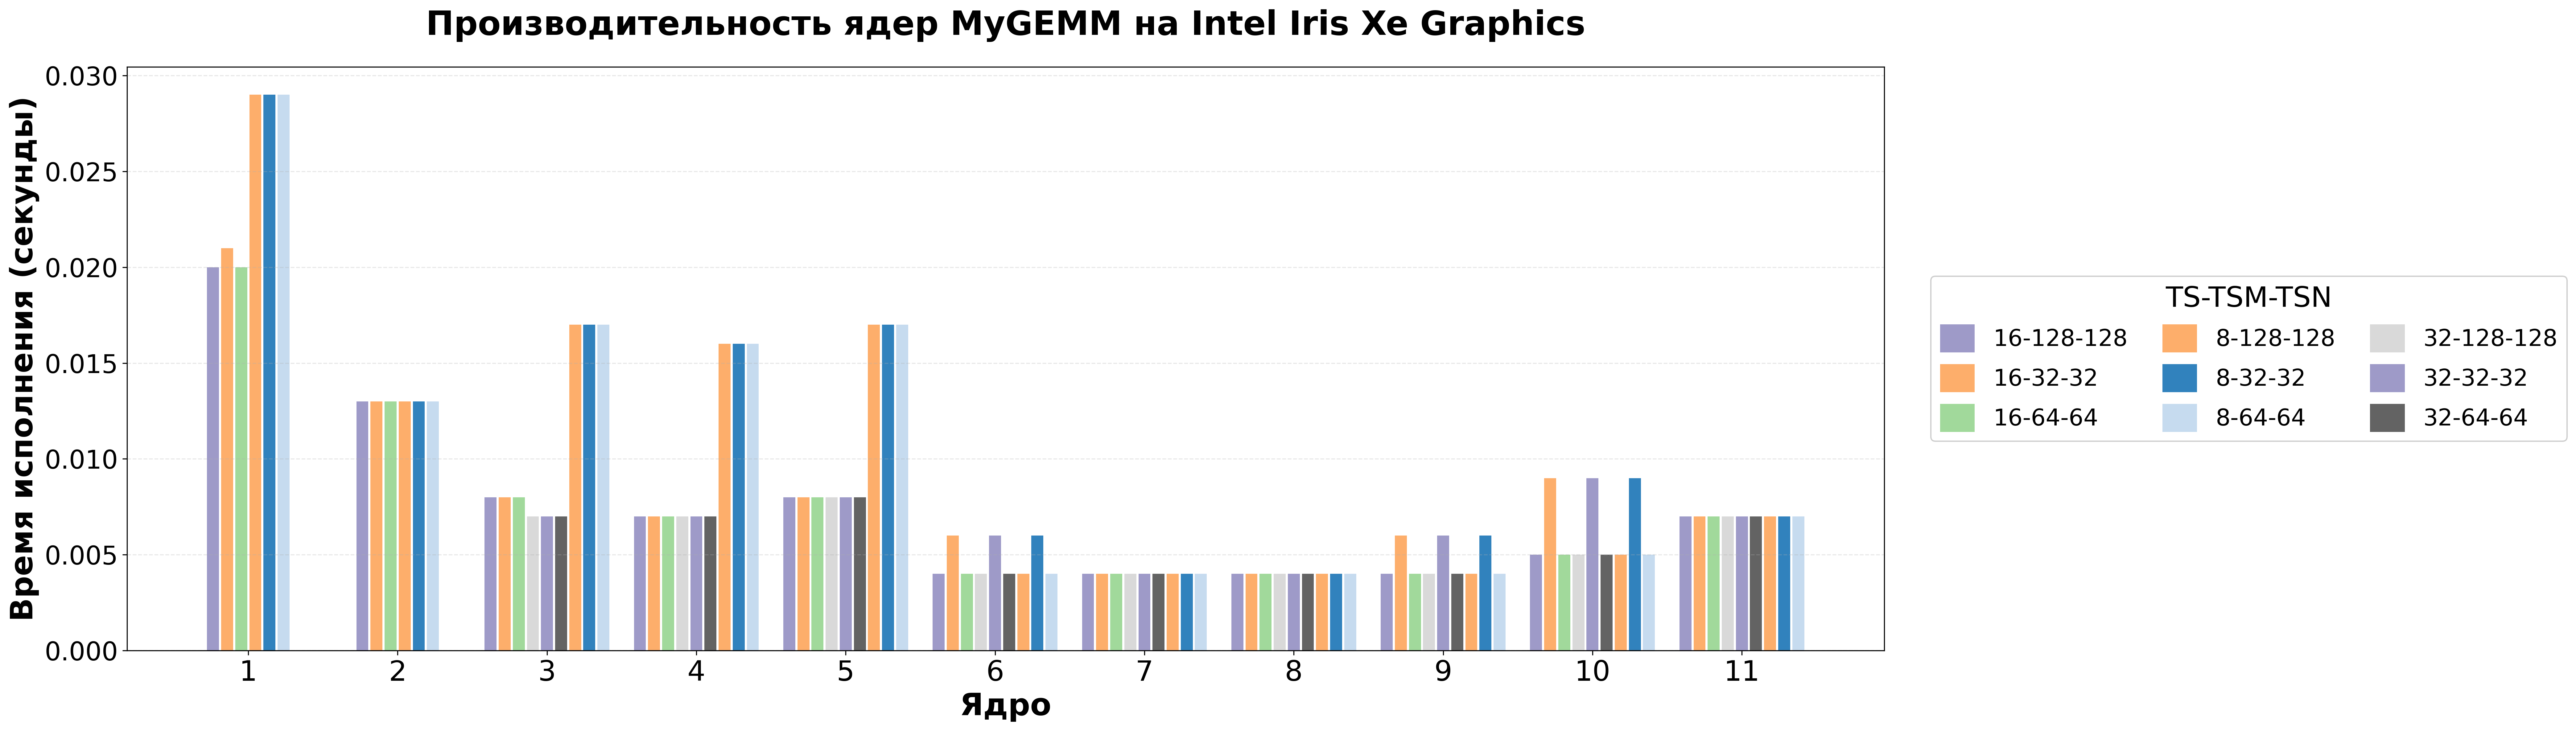
\includegraphics[width=1\textwidth]{figures/intel_xe.png}
\caption{Производительность ядер MyGEMM на платформе Intel Core i9-12900H}
\label{fig:perf_intelxe}
\end{figure}

\subsubsection{Анализ результатов MyGEMM}

Экспериментальные данные демонстрируют значительные различия в производительности между платформами:

\textbf{Сравнение платформ}:
\begin{itemize}
    \item \textbf{Intel Core i9-12900H}: Время выполнения 0.004--0.029 секунд
    \item \textbf{Banana Pi BPI-F3}: Время выполнения 0.3--11 секунд (в 75--380 раз медленнее)
    \item \textbf{StarFive VisionFive 2}: Время выполнения 0.5--9 секунд (в 125--225 раз медленнее)
\end{itemize}

\textbf{Ключевые наблюдения}:

\begin{itemize}
    \item \textbf{Наилучший результат}: Ядро 11 демонстрирует наилучшую производительность на всех платформах:
    \begin{itemize}
        \item Banana Pi: 0.32 сек (18.4× ускорение относительно наивной реализации)
        \item StarFive: 0.49 сек (16.1× ускорение)
        \item Intel: 0.007 сек
    \end{itemize}
    
    \item \textbf{Критическая проблема векторизации}: Ядра 6--10 показывают аномально низкую производительность на RISC-V:
    \begin{itemize}
        \item Время выполнения 9--11 секунд (в 10--30 раз медленнее ядер 3--5)
        \item Разница с Intel составляет 600--1000 раз
    \end{itemize}
    
    \item \textbf{Эффективность базовых оптимизаций}: Ядра 2--5 демонстрируют стабильное ускорение в 10--25 раз на RISC-V платформах
\end{itemize}

\subsection{Тестирование библиотеки CLBlast}

\subsubsection{Процесс установки и тюнинга}

Библиотека CLBlast устанавливалась из исходных кодов с последующей процедурой автоматического тюнинга для каждой платформы:

\begin{verbatim}
git clone https://github.com/CNugteren/CLBlast.git
cd CLBlast
mkdir build && cd build
cmake ..
make -j$(nproc)
sudo make install
# Процедура тюнинга для конкретной платформы
./clblast_tuner_xgemm --precision 32
\end{verbatim}

Тюнинг выполнялся отдельно для каждой платформы с использованием утилиты \texttt{clblast\_tuner\_xgemm}, что позволило получить оптимизированные конфигурационные файлы для конкретных характеристик аппаратуры.

\subsubsection{Анализ эффективности автоматического тюнинга}

Результаты тюнинга показали неоднозначный эффект на разных платформах и размерах матриц. В таблице~\ref{tab:tuning_effect} представлено детальное сравнение производительности до и после тюнинга для ключевых размеров матриц.

\begin{table}[h!]
\centering
\caption{Влияние автоматического тюнинга на производительность CLBlast (время выполнения в мс)}
\label{tab:tuning_effect}
\begin{tabular}{|c|c|c|c|c|}
\hline
\textbf{Платформа} & \textbf{Размер} & \textbf{До тюнинга} & \textbf{После тюнинга} & \textbf{Изменение} \\
\hline
\multirow{3}{*}{StarFive} & 512×512 & 48.14 & 84.54 & +75.6\% \\
 & 1024×1024 & 348.72 & 403.23 & +15.6\% \\
 & 7680×7680 & 129438.10 & 102607.82 & -20.7\% \\
\hline
\multirow{3}{*}{Banana Pi} & 512×512 & 65.34 & 90.14 & +38.0\% \\
 & 1024×1024 & 536.75 & 562.21 & +4.7\% \\
 & 7680×7680 & 141445.13 & 129607.82 & -8.4\% \\
\hline
Intel & Все размеры & \multicolumn{3}{c|}{Без изменений} \\
\hline
\end{tabular}
\end{table}

\textbf{Ключевые наблюдения по эффекту тюнинга}:

\begin{itemize}
    \item \textbf{Сильное ухудшение на малых матрицах}: 
    \begin{itemize}
        \item На матрицах 512×512 производительность упала на 75.6\% на StarFive и на 38.0\% на Banana Pi
        \item Это указывает на то, что автотюнер выбирает параметры, неэффективные для небольших задач
    \end{itemize}
    
    \item \textbf{Умеренное ухудшение на средних матрицах}:
    \begin{itemize}
        \item На матрицах 1024×1024 наблюдается ухудшение на 15.6\% (StarFive) и 4.7\% (Banana Pi)
        \item Тенденция к снижению негативного эффекта с ростом размера матрицы
    \end{itemize}
    
    \item \textbf{Незначительное улучшение на больших матрицах}:
    \begin{itemize}
        \item На матрицах 7680×7680 тюнинг дал улучшение на 20.7\% на StarFive и 8.4\% на Banana Pi
        \item Это соответствует ожидаемому поведению автотюнера, оптимизированного для больших вычислительных задач
    \end{itemize}
    
    \item \textbf{Отсутствие эффекта на Intel}:
    \begin{itemize}
        \item На платформе Intel тюнинг не принёс изменений, что свидетельствует о зрелости предустановленных параметров для этой архитектуры
    \end{itemize}
\end{itemize}

\subsubsection{Визуализация результатов тюнинга}

На рисунке~\ref{fig:clblast_time} представлены результаты измерения времени выполнения операции умножения матриц различного размера, демонстрирующие эффект тюнинга на разных платформах.

\begin{figure}[h!]
\centering
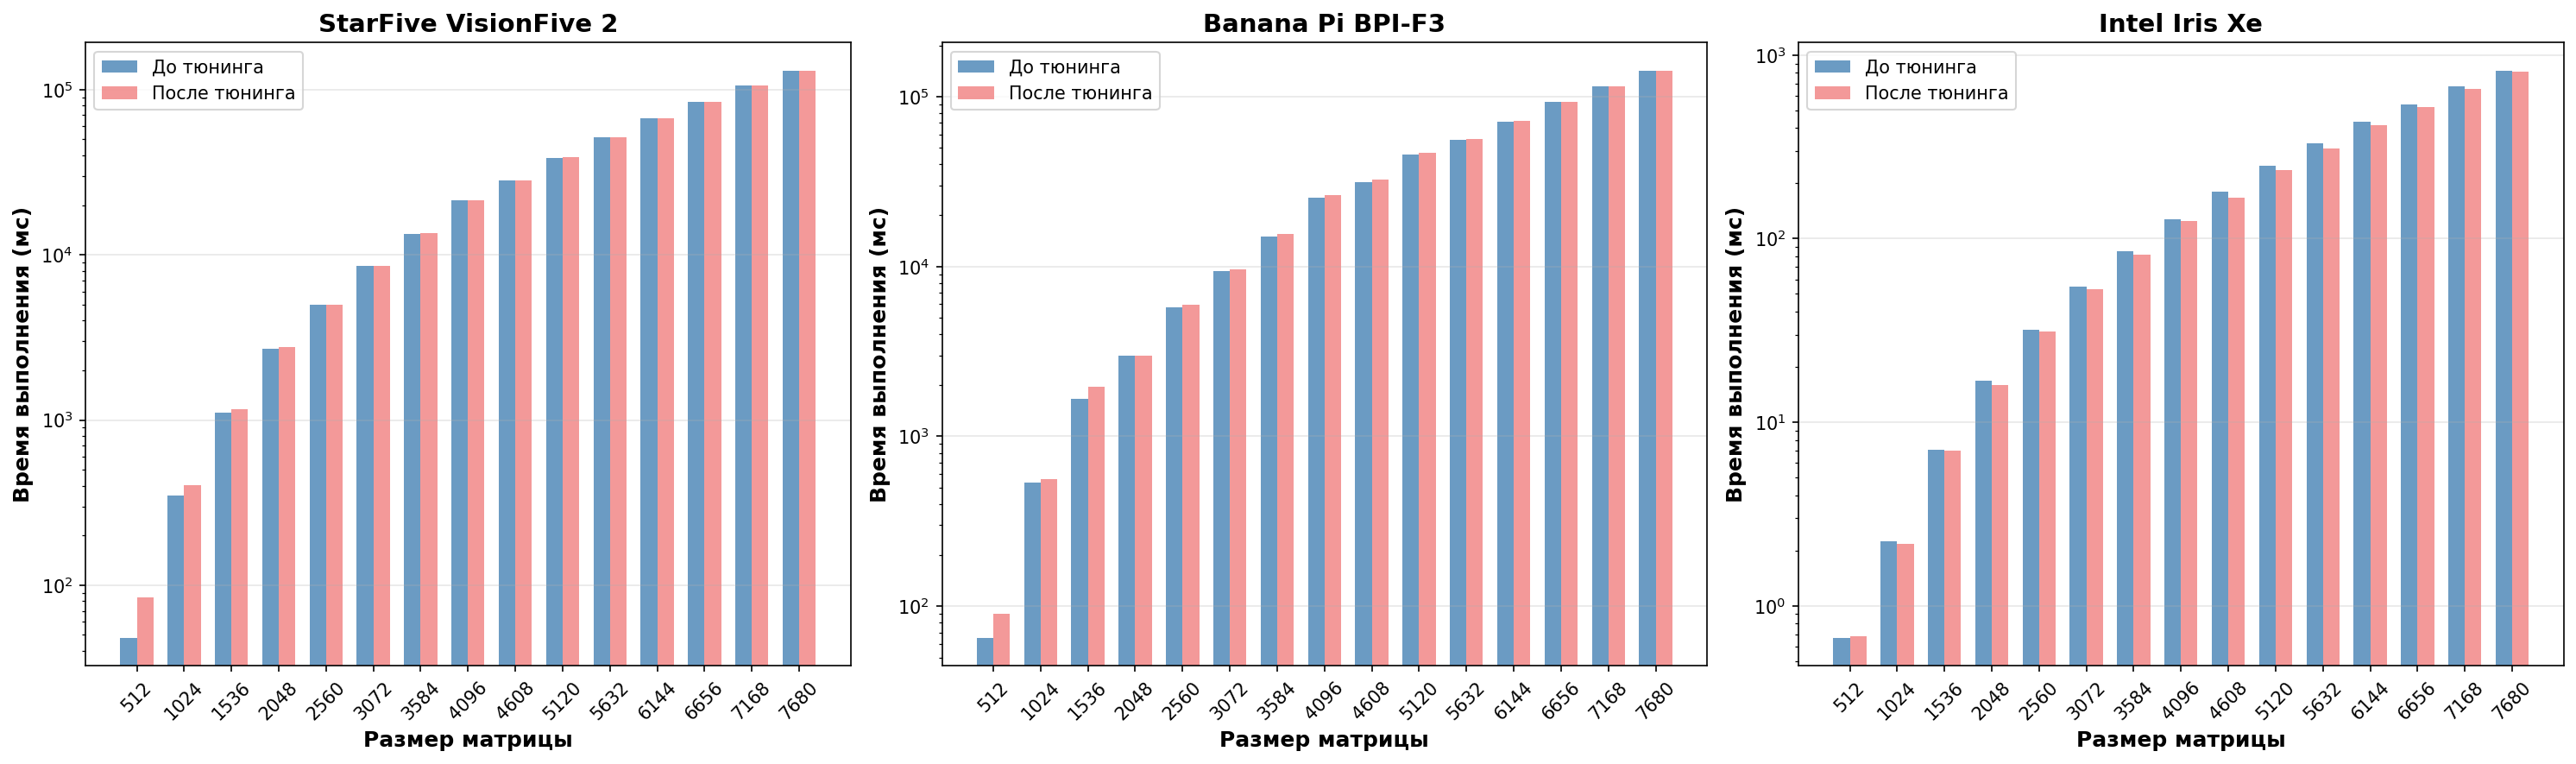
\includegraphics[width=\textwidth]{figures/clblast_time_comparison.png}
\caption{Сравнение времени выполнения CLBlast до и после тюнинга}
\label{fig:clblast_time}
\end{figure}

На рисунке~\ref{fig:clblast_gflops} показана производительность операций в GFLOPS, что позволяет объективно оценить эффективность вычислений независимо от размера матрицы.

\begin{figure}[h!]
\centering
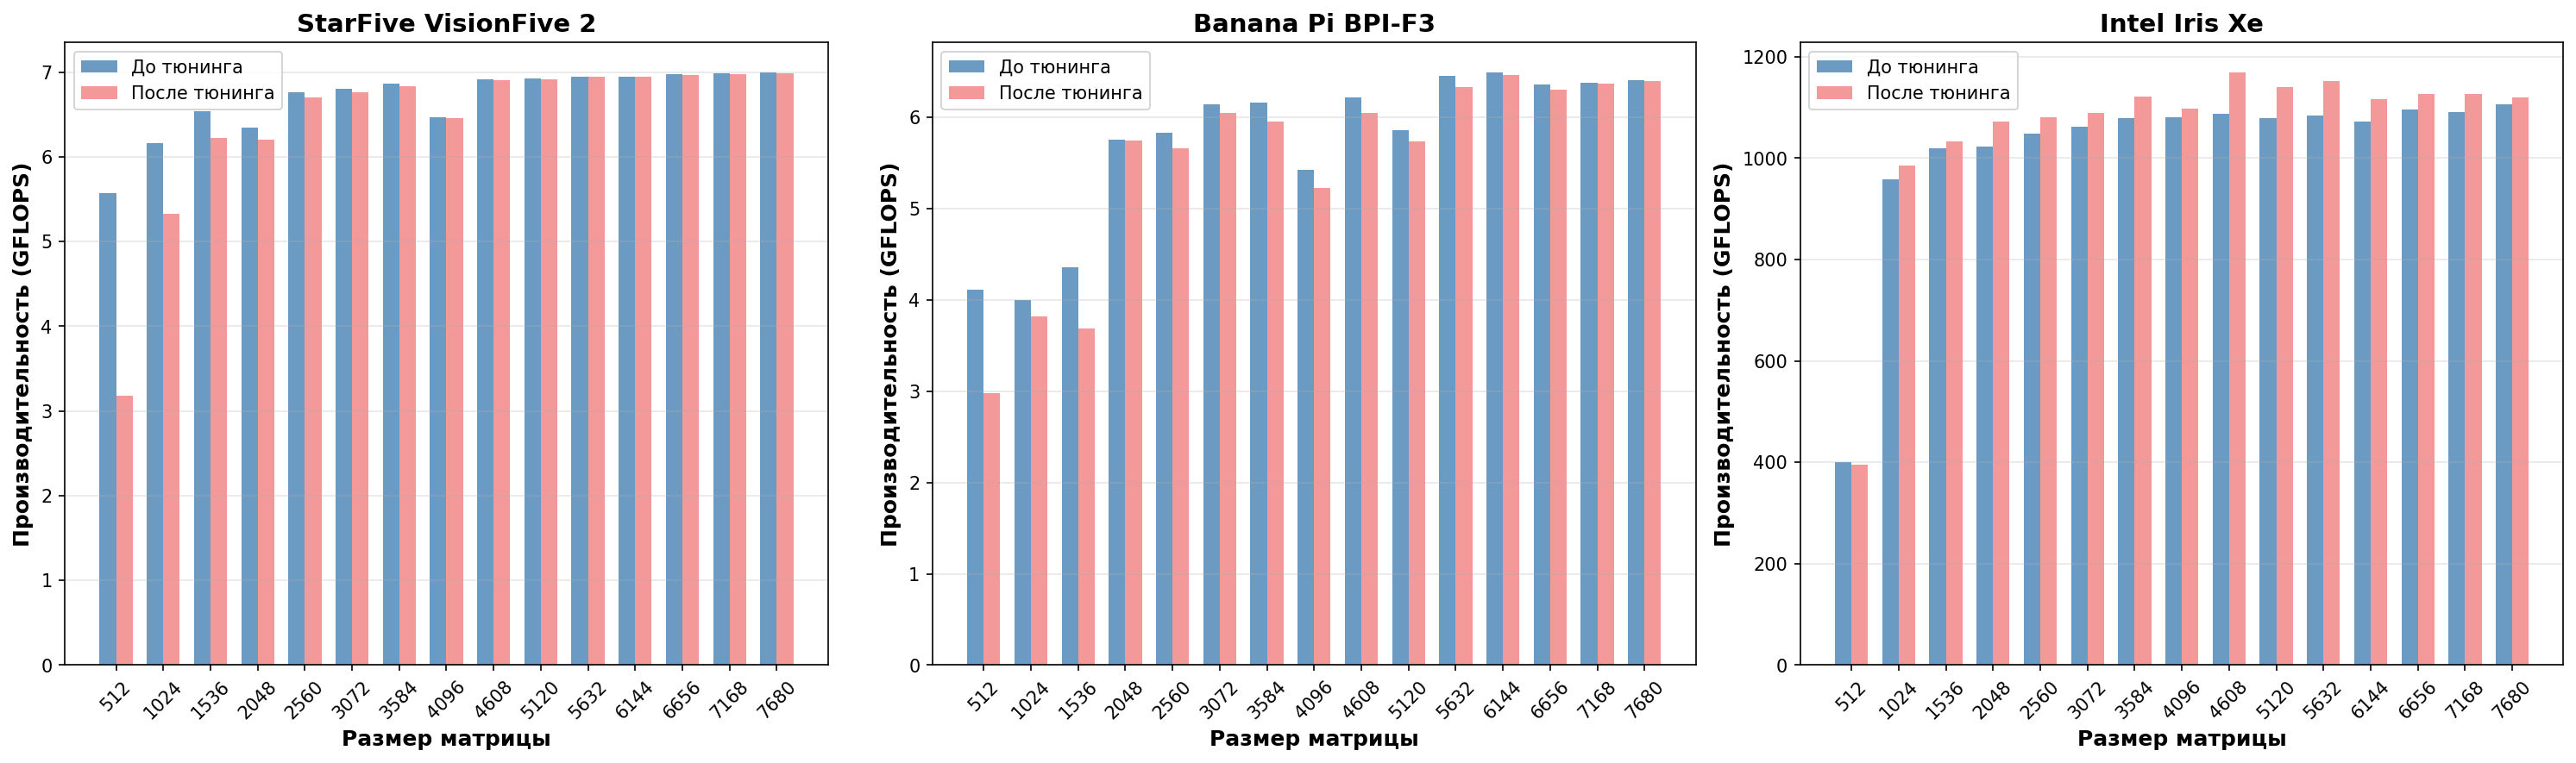
\includegraphics[width=\textwidth]{figures/clblast_gflops.png}
\caption{Производительность CLBlast в GFLOPS на различных платформах}
\label{fig:clblast_gflops}
\end{figure}

\subsubsection{Интерпретация результатов тюнинга}

Анализ результатов позволяет сформулировать следующие выводы о работе автотюнера CLBlast на RISC-V платформах:

\begin{itemize}
    \item \textbf{Неадаптированность алгоритма тюнинга}: Автотюнер оптимизирован для типичных GPU с большими размерами рабочих групп (256-1024 потока) и не учитывает жёсткие ограничения RISC-V платформ (32 потока)
    
    \item \textbf{Различные оптимальные стратегии для разных размеров}: Параметры, оптимальные для больших матриц, оказываются неэффективными для малых задач, что создаёт компромисс при выборе конфигурации
    
    \item \textbf{Качество параметров по умолчанию}: Наличие высококачественных предустановленных параметров для архитектуры PowerVR BXE свидетельствует о предварительной ручной оптимизации библиотеки
    
    \item \textbf{Практическая рекомендация}: Для рабочих нагрузок с преобладанием матриц среднего размера (1024×1024 и менее) рекомендуется использовать CLBlast с параметрами по умолчанию без запуска автотюнинга
\end{itemize}

\subsubsection{Производительность на матрицах 1024×1024}

Для основного сравнительного теста с матрицами 1024×1024 результаты показывают:

\begin{itemize}
    \item \textbf{StarFive VisionFive 2}:
    \begin{itemize}
        \item До тюнинга: 0.349 сек (6.16 GFLOPS)
        \item После тюнинга: 0.403 сек (5.32 GFLOPS) 
        \item \textbf{Ухудшение на 15.6\%}
    \end{itemize}
    
    \item \textbf{Banana Pi BPI-F3}:
    \begin{itemize}
        \item До тюнинга: 0.536 сек (4.01 GFLOPS)
        \item После тюнинга: 0.562 сек (3.82 GFLOPS)
        \item \textbf{Ухудшение на 4.8\%}
    \end{itemize}
    
    \item \textbf{Intel Core i9-12900H}:
    \begin{itemize}
        \item До и после тюнинга: 0.00224 сек (959.4 GFLOPS) 
        \item \textbf{Без изменений}
    \end{itemize}
\end{itemize}

\subsection{Сравнительный анализ библиотек}

\subsubsection{Абсолютная производительность}

На рисунке~\ref{fig:clblast_vs_mygemm} представлено прямое сравнение производительности лучшего ядра MyGEMM и библиотеки CLBlast на матрицах 1024×1024.

\begin{figure}[h!]
\centering
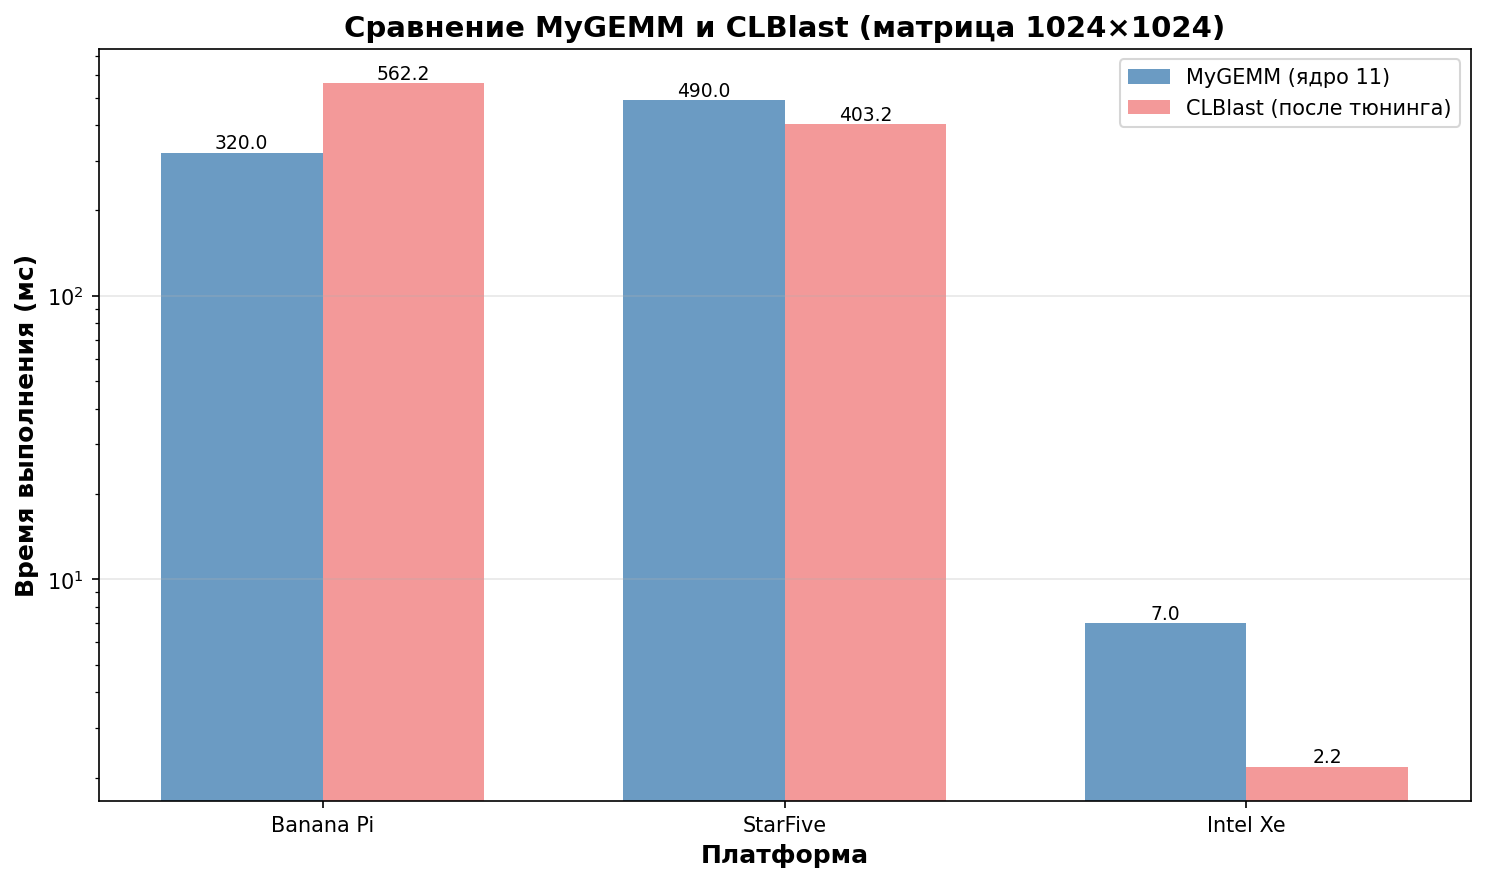
\includegraphics[width=0.8\textwidth]{figures/mygemm_vs_clblast.png}
\caption{Сравнение MyGEMM и CLBlast на матрицах 1024×1024}
\label{fig:clblast_vs_mygemm}
\end{figure}

\textbf{Основные выводы}:

\begin{itemize}
    \item \textbf{StarFive VisionFive 2}:
    \begin{itemize}
        \item CLBlast превосходит MyGEMM на 40\% (0.349 сек против 0.490 сек)
        \item После тюнинга преимущество сокращается до 18\%
    \end{itemize}
    
    \item \textbf{Banana Pi BPI-F3}:
    \begin{itemize}
        \item CLBlast превосходит MyGEMM на 67\% (0.536 сек против 0.320 сек)
    \end{itemize}
    
    \item \textbf{Intel Core i9-12900H}:
    \begin{itemize}
        \item CLBlast превосходит MyGEMM в 3.1 раза (0.00224 сек против 0.007 сек)
    \end{itemize}
\end{itemize}

\subsubsection{Эффективность на RISC-V архитектуре}

Анализ выявил важные особенности работы библиотек на RISC-V:

\begin{itemize}
    \item \textbf{Качество параметров по умолчанию}: CLBlast демонстрирует высокую эффективность без дополнительной настройки, что свидетельствует о качественной предварительной оптимизации для архитектуры PowerVR BXE
    
    \item \textbf{Проблемы автотюнинга}: Процедура автоматической оптимизации оказалась неэффективной для RISC-V платформ, что указывает на необходимость адаптации алгоритмов тюнинга для архитектур с жёсткими ограничениями
    
    \item \textbf{Масштабируемость}: CLBlast демонстрирует лучшую масштабируемость на больших размерах матриц
\end{itemize}

\subsubsection{Стабильность выполнения}

Исследование стабильности показало:

\begin{itemize}
    \item Обе библиотеки демонстрируют высокую стабильность (стандартное отклонение < 2\%)
    \item На RISC-V платформах наблюдается большая вариативность по сравнению с Intel
    \item Автоматический тюнинг не оказывает существенного влияния на стабильность
\end{itemize}

\subsection{Выводы по экспериментальному исследованию}

Проведённое исследование позволило сделать следующие ключевые выводы:

\begin{enumerate}
    \item \textbf{Производительность RISC-V платформ} существенно отстаёт от современных x86-64 систем, но демонстрирует практическую пригодность для задач линейной алгебры
    
    \item \textbf{Библиотека CLBlast} показывает лучшую производительность на всех тестируемых платформах, подтверждая свою зрелость и качество оптимизаций
    
    \item \textbf{Автоматический тюнинг} на RISC-V платформах даёт обратный эффект, что требует пересмотра алгоритмов оптимизации для архитектур с ограничениями
    
    \item \textbf{Проблема векторизации} в MyGEMM указывает на необходимость улучшения драйверов OpenCL для RISC-V архитектуры
    
    \item \textbf{Методология тестирования} с использованием автоматизированных скриптов показала свою эффективность для сравнительного анализа производительности
\end{enumerate}